\documentclass{article}
\usepackage[utf8]{inputenc}
\usepackage[includeheadfoot, margin=1em,headheight=2em]{geometry}
\usepackage{titling}
\geometry{a4paper, left=2cm, right=2cm, top=2cm, bottom=2cm}
\usepackage{graphicx}
\usepackage{float}
\providecommand{\versionnumber}{1.0.0}
\usepackage{enumitem}
\usepackage{array}
\usepackage[italian]{babel}
\newcolumntype{P}[1]{>{\centering\arraybackslash}p{#1}}
\renewcommand{\arraystretch}{1.5} % Default value: 1
\setlength{\droptitle}{-6em}

%font
\usepackage[defaultfam,tabular,lining]{montserrat}
\usepackage[T1]{fontenc}
\renewcommand*\oldstylenums[1]{{\fontfamily{Montserrat-TOsF}\selectfont #1}}

%custom bold 
\usepackage[outline]{contour}
\usepackage{xcolor}
\newcommand{\custombold}{\contour{black}}

%table colors
\usepackage{color, colortbl}
\definecolor{Blue}{rgb}{0.51,0.68,0.79}
\definecolor{LightBlue}{rgb}{0.82,0.87,0.90}
\definecolor{LighterBlue}{rgb}{0.93,0.95,0.96}

%Header
\usepackage{fancyhdr, xcolor}
\pagestyle{fancy}
\let\oldheadrule\headrule% Copy \headrule into \oldheadrule
\renewcommand{\headrule}{\color{Blue}\oldheadrule}% Add colour to \headrule
\renewcommand{\headrulewidth}{0.2em}
\fancyhead[L]{Studio ARIS}
\fancyhead[C]{Samuele Vignotto}
\fancyhead[R]{
\includegraphics[height=1cm]{Logo/Y_LOGO-SOLO.png}}
\setcounter{secnumdepth}{0}

\title{\Huge{\textbf{ARIS}}\vspace{-1em}}
\author{Samuele Vignotto}
\date{}
\begin{document}
\maketitle
\begin{figure}[h]
  \centering
  
\includegraphics[width=6cm, height=6cm]{Logo/Y_LOGO-SOLO.png}
  \label{fig:immagine}
\end{figure}

\newpage
\tableofcontents
\newpage

\section{Introduzione}
ARIS Process Mining è uno strumento progettato per supportare le organizzazioni nell'analisi e nell'ottimizzazione dei propri processi aziendali. Sviluppato da Software AG, ARIS Process Mining offre una profonda comprensione del modo in cui i processi vengono effettivamente eseguiti all'interno di un'organizzazione, analizzando i dati storici raccolti da vari sistemi aziendali e ricostruendo i flussi di lavoro reali. Questo consente di identificare inefficienze, colli di bottiglia e deviazioni rispetto ai processi ideali o pianificati. Una delle principali caratteristiche di ARIS è la capacità di visualizzare in modo dettagliato e intuitivo i processi aziendali. Attraverso dashboard interattive e rappresentazioni grafiche avanzate, gli utenti possono ottenere una visione completa del ciclo di vita dei processi, evidenziando le aree critiche che necessitano di miglioramenti. ARIS si distingue anche per le sue potenti funzionalità di analisi, che includono il monitoraggio continuo delle performance dei processi e l'identificazione automatica di anomalie. Grazie alla sua integrazione con altre piattaforme e tecnologie di automazione, ARIS facilita la creazione di processi automatizzati e promuove la digitalizzazione delle operazioni aziendali, riducendo l'intervento umano e migliorando l'efficienza operativa. Inoltre, ARIS Process Mining supporta funzionalità di simulazione avanzate che consentono di testare scenari di ottimizzazione e prevedere l'impatto di eventuali modifiche sui processi aziendali. Questo approccio basato sui dati migliora la capacità decisionale dell'azienda, permettendo un'implementazione più efficace di strategie di ottimizzazione e trasformazione digitale.

\section{Formati dei dati supportati}

\subsection{CSV (Comma-Separated Values)}
Utilizzato per l'importazione e l'esportazione di dati di origine. È il formato principale per caricare dati da sistemi aziendali e fonti esterne.

\section{Fonti di dati supportate}
\subsection{SAP}
ARIS Process Mining è strettamente integrato con i sistemi SAP, permettendo l'estrazione dei dati di processo direttamente dai sistemi ERP di SAP. Questa integrazione consente di analizzare i processi aziendali senza la necessità di esportare manualmente i dati.
\subsection{JDBC (Java Database Connectivity)}
ARIS supporta JDBC per la connessione diretta a vari database relazionali, come Oracle, Microsoft SQL Server e altri database compatibili. Questa connessione consente di estrarre in tempo reale i dati necessari per l'analisi dei processi.
\subsection{Data ingestion API}
ARIS offre un'opzione avanzata di connessione tramite API, che consente di estrarre dati da diverse fonti esterne. Questo amplia notevolmente le possibilità di integrazione, permettendo di collegarsi a numerosi sistemi aziendali o applicazioni.

\section{Funzionalità}
\subsection{Process overview}
La funzionalità Process Overview di ARIS fornisce la possibilità di accedere alle metriche chiave che offrono informazioni essenziali per l'analisi dei processi. Tra queste, vi sono il numero di casi e il tempo medio di esecuzione.\\
Inoltre, l'interfaccia è altamente interattiva, permettendo agli utenti di filtrare le informazioni per ottenere approfondimenti mirati e identificare eventuali anomalie o variazioni.
\subsection{Process Explorer}
La funzionalità Process Explorer di ARIS Process Mining offre una rappresentazione interattiva e visiva dei processi aziendali, permettendo di esplorarli in modo dettagliato. Questo strumento consente agli utenti di visualizzare le diverse fasi del processo, identificare varianti e analizzare le connessioni tra le attività eseguite.\\
Una delle caratteristiche principali di Process Explorer è la capacità di esplorare le varianti del processo, il che consente di individuare eventuali deviazioni dal flusso di lavoro standard o inefficienze operative. Questo strumento è utile per identificare punti di blocco, analizzare i colli di bottiglia e confrontare i processi reali con quelli pianificati. Inoltre, integra funzionalità di filtraggio che permettono agli utenti di concentrarsi su specifici passaggi o metriche del processo, facilitando una diagnosi mirata dei problemi.
\subsection{Compliance}
La funzionalità Compliance di ARIS Process Mining permette di monitorare l'aderenza dei processi aziendali rispetto a modelli predefiniti e alle regole operative stabilite. Questa funzionalità consente di confrontare l'esecuzione effettiva dei processi con il modello teorico, verificando che siano seguiti correttamente i passaggi stabiliti dalle politiche aziendali e dalle normative.\\
Il processo di verifica avviene attraverso il confronto con modelli di processo definiti in linguaggi come BPMN. ARIS analizza il flusso delle attività e genera metriche di conformità, fornendo un "compliance rate" che indica la percentuale di casi che seguono correttamente il processo definito. In caso di violazioni, il sistema segnala dove avvengono deviazioni rispetto alle regole stabilite, permettendo di identificare e correggere eventuali inefficienze o potenziali rischi di non conformità.
\subsection{App Builder}
La funzionalità App Builder di ARIS Process Mining consente agli utenti di creare applicazioni personalizzate per l'analisi dei processi aziendali. Questa funzione è estremamente versatile e permette di combinare diversi componenti grafici, come grafici, tabelle e KPI, per costruire dashboard personalizzate che rispondano a esigenze specifiche dell'organizzazione.\\
L'App Builder supporta la creazione di colonne calcolate direttamente all'interno dell'applicazione, permettendo di eseguire calcoli su variabili e KPI senza dover ricaricare i dati.

\section{Implementazioni pratiche: simulazione}
Il file CSV è stato creato mediante uno script Python che simula una serie di attività relative alla produzione e alla gestione degli ordini di prodotti. Inoltre, per la simulazione dei dati, sono stati presi in considerazione anche i dati estratti manualmente da un database di un sistema gestionale.
\subsection{Regole di simulazione}
\subsubsection{Impostazione delle date iniziali}
Ogni ciclo di attività inizia con la prima attività programmata tra il 1 gennaio 2019 e il 31 dicembre 2020.\\
\subsubsection{Definizione delle tipologie di prodotti}
Viene creata una lista di 30 tipi di scarpe, denominate "Scarpe tipo 1" fino a "Scarpe tipo 30".\\
\subsubsection{Definizione delle attività e delle durate}
Sono state definite 17 attività, ciascuna con un ID unico e una durata variabile. Le durate delle attività sono espresse in minuti o giorni, a seconda dell'attività specifica.\\
\subsubsection{Generazione di un ciclo di attività per prodotto}
Per ciascun prodotto, viene generato un ciclo di attività che segue le seguenti regole:
\begin{itemize}
    \item \custombold{attività obbligatorie}: alcune attività avvengono in un ordine fisso. Ad esempio, "Conferma ordine" è sempre seguita da "Creazione progetto";
    \item \custombold{modifica del progetto}: un numero casuale di modifiche al progetto (da 1 a 5) può essere aggiunto dopo la creazione del progetto;
    \item \custombold{gestione degli ordini fornitore}: un numero casuale (da 1 a 3) di cicli di gestione ordini fornitore può essere inserito, ognuno dei quali può includere attività come "Ordine fornitore", "Arrivo offerta fornitore", "Ordine annullato" o "Ordine sospeso";
    \item \custombold{produzione}: vengono aggiunte attività relative alla produzione, come "Stampa scheda di produzione", "Inizio ciclo di produzione" e "Termine ordine di produzione";
    \item \custombold{attività non necessarie}: possono essere inserite attività opzionali come "Controllo qualità non necessario" (20\% di probabilità) e "Ri-lavorazione non necessaria" (10\% di probabilità);
    \item \custombold{consegna}: dopo la produzione, viene aggiunta l'attività di "Consegna".
\end{itemize}
\subsubsection{Generazione dei timestamp}
Ogni attività riceve un timestamp generato casualmente basato su un intervallo di tempo definito per quella specifica attività.
\subsubsection{Ciclo di generazione dei dati}
Il numero di prodotti varia tra 300 e 500, determinato casualmente. Per ogni prodotto, viene generato un ciclo di attività completo, assicurandosi che tutte le attività obbligatorie siano inserite nel corretto ordine e che le attività casuali siano distribuite come specificato.\\
\subsubsection{Mischiamento casuale delle righe del file CSV}
È stato utilizzato un algoritmo per mischiare in modo casuale le righe del file CSV. L'algoritmo legge il file CSV originale e separa l'intestazione dai dati. Successivamente, le righe dei dati vengono mescolate casualmente mantenendo intatta l'intestazione. Infine, il nuovo file CSV, con le righe mescolate, viene salvato in un file di output. Questo processo assicura che i dati siano riorganizzati in modo casuale senza alterare la struttura del file CSV.

\subsection{Process explorer}
\begin{figure}[H]
    \centering
    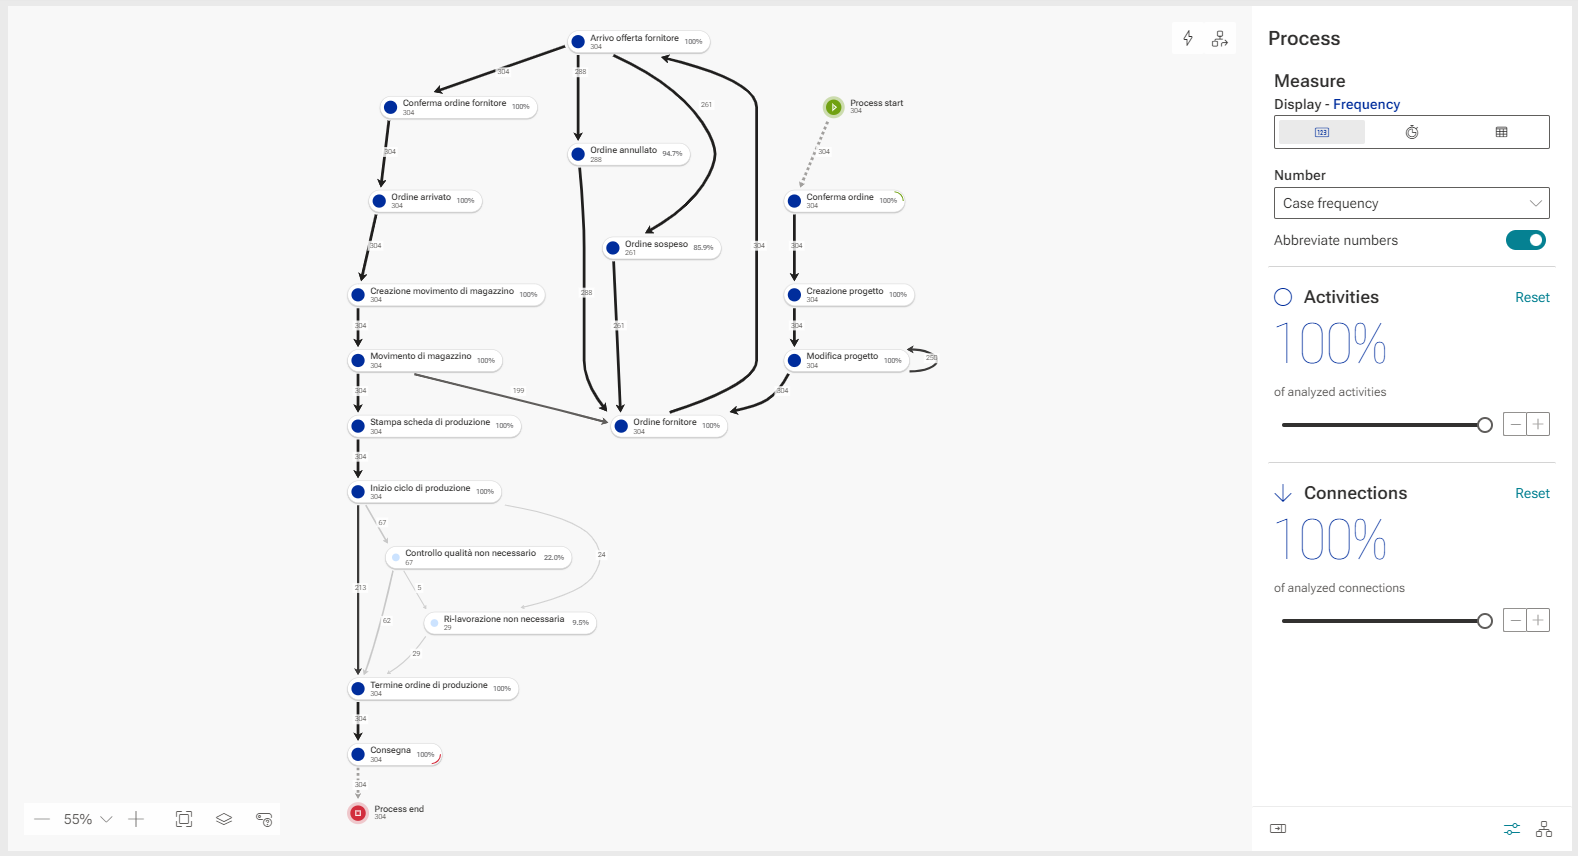
\includegraphics[width=\textwidth]{imgARIS/Simulazione/ProcessExplorerSimulazione.png}
    \caption{Mappa del processo}
    \label{fig:process-map}
\end{figure}
Quello che si vede al centro della schermata è una mappa che rappresenta un intero processo aziendale. Ogni cerchio nella mappa indica un'attività specifica, come la "Conferma ordine fornitore" o la "Consegna", mentre le frecce che collegano questi cerchi rappresentano la sequenza delle operazioni e la direzione del flusso. Queste frecce mostrano chiaramente come si passa da un'attività all'altra, e il numero sopra di esse fornisce una visione quantitativa del flusso, indicando quante volte un determinato passaggio è avvenuto. Più la freccia è spessa, più frequentemente viene eseguito quel passaggio, il che aiuta immediatamente a identificare quali parti del processo sono le più comuni e dove, invece, ci sono varianti meno frequenti.\\
Guardando la parte destra della schermata, troviamo la sezione delle misure. Qui, in particolare, si evidenzia la "frequenza dei casi", che ci mostra quante volte un'attività è stata eseguita. Questo strumento permette di osservare non solo quanto spesso si verificano determinati passaggi, ma consente anche di personalizzare la visualizzazione dei dati, permettendo ad esempio di visualizzare il tempo impiegato in ciascuna fase del processo, non solo la frequenza.\\
ARIS Process Explorer offre, inoltre, la possibilità di analizzare l’interezza del processo o solo porzioni di esso. Nella sezione “Activities” e “Connections” possiamo osservare come sia stato analizzato il 100\% delle attività e delle connessioni, ma l'utente può ridurre questo numero per concentrarsi su specifici aspetti del processo.

\subsection{Process overview}
\begin{figure}[H]
    \centering
    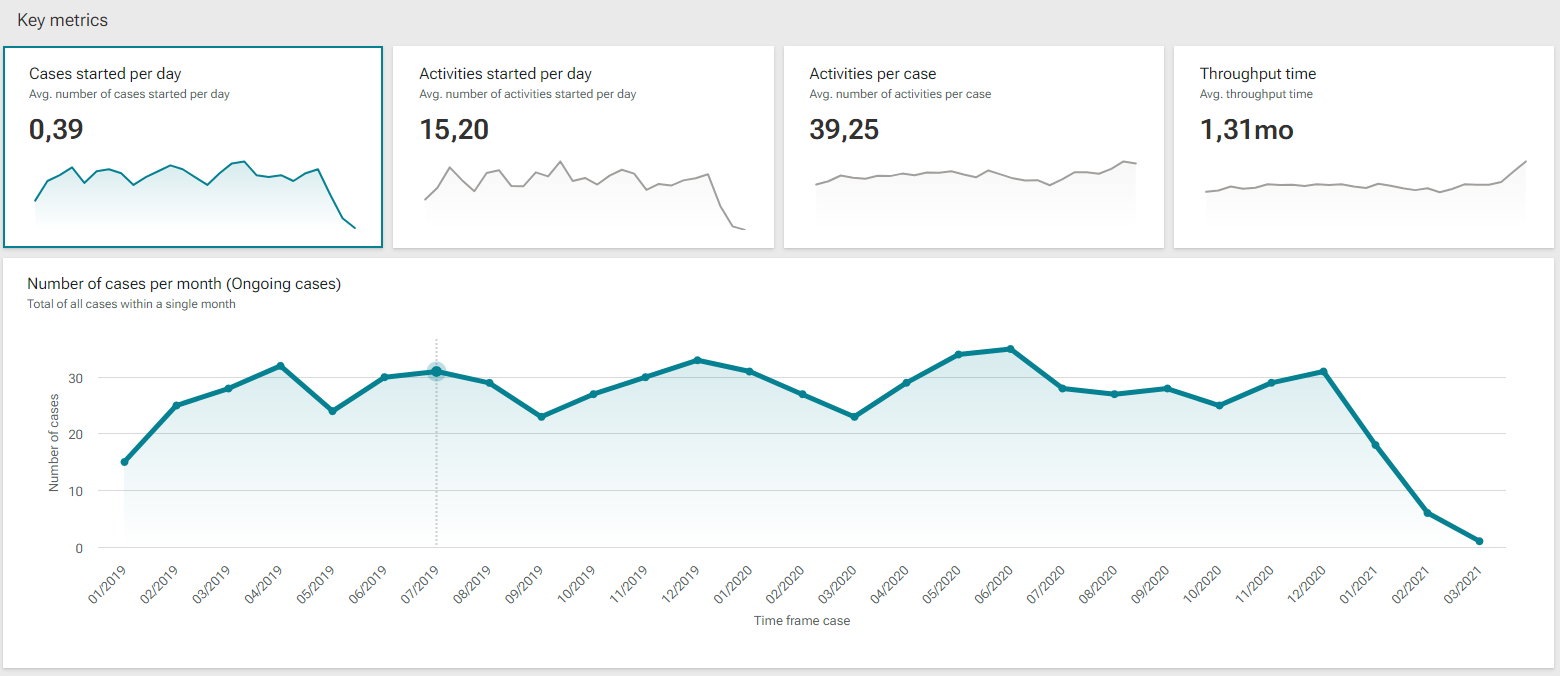
\includegraphics[width=\textwidth]{imgARIS/Simulazione/ProcessOverview1Simulazione.png}
    \caption{Panoramica delle metriche chiave del processo}
    \label{fig:process-overview-1}
\end{figure}
Questa schermata offre una sintesi intuitiva delle performance complessive del processo attraverso una serie di metriche chiave e visualizzazioni grafiche. Ad esempio, i Key Metrics forniscono un’istantanea del processo. Le metriche come il numero di casi iniziati giornalmente, il numero di attività avviate e il tempo di attraversamento medio permettono di farsi un'idea immediata della salute del processo. Ciò che rende questa funzionalità particolarmente utile è la sua capacità di aggregare dati complessi in pochi indicatori sintetici, rendendo facilmente accessibili informazioni che altrimenti potrebbero richiedere lunghe analisi manuali.\\
Un altro aspetto interessante è il grafico del numero di casi mensili, che non è solo una rappresentazione statica, ma permette di visualizzare come il processo si evolve nel tempo. Questo è cruciale per comprendere trend stagionali o variazioni nella domanda, e per vedere l’impatto di eventuali modifiche nei processi o nelle politiche aziendali.\\
\begin{figure}[H]
    \centering
    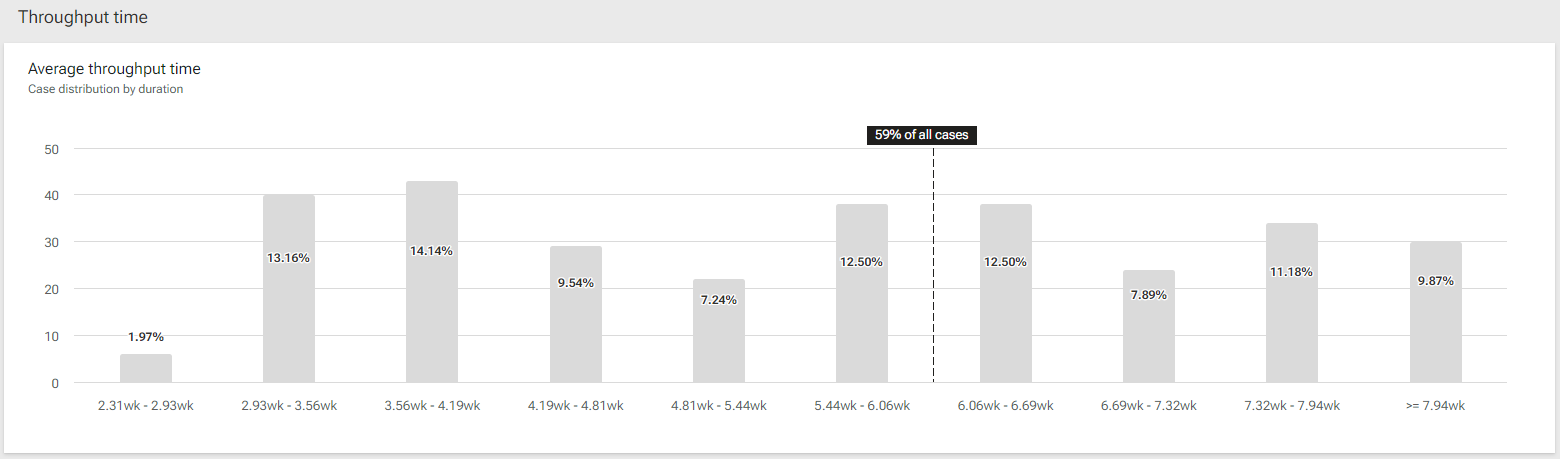
\includegraphics[width=\textwidth]{imgARIS/Simulazione/ProcessOverview2Simulazione.png}
    \caption{Distribuzione del tempo di attraversamento dei casi}
    \label{fig:process-overview-2}
\end{figure}
il grafico relativo al tempo di attraversamento ci fornisce una distribuzione dei tempi impiegati per completare i vari casi. Questo tipo di visualizzazione è particolarmente utile quando si vuole capire la variabilità nel processo. È infatti possibile vedere chiaramente quali casi vengono completati in tempi brevi e quali richiedono più tempo del previsto. Questa visione granulare permette all’utente di focalizzarsi non solo sulla media, ma anche sulle eccezioni, ovvero quei casi che impiegano molto più tempo del normale. Una distribuzione ben visibile come quella mostrata aiuta a individuare facilmente le categorie di tempo più critiche, consentendo di indirizzare le azioni di miglioramento in modo mirato.

\subsection{App builder}
\begin{figure}[H]
    \centering
    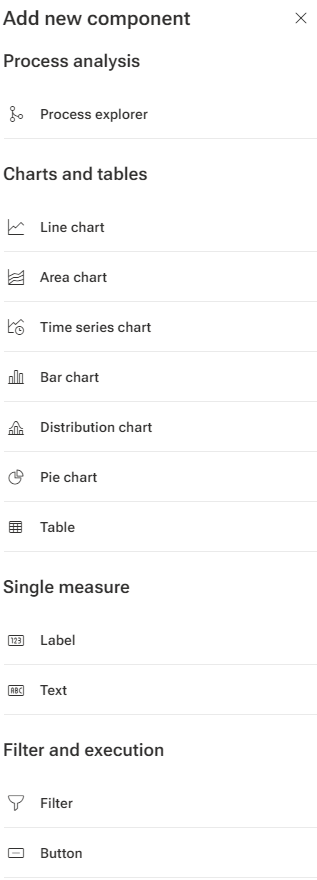
\includegraphics{imgARIS/Simulazione/AppBuilderSimulazione.png}
    \caption{Opzioni disponibili per l'App builder}
    \label{fig:options-app-builder}
\end{figure}
La prima opzione è il Process Explorer, che offre la possibilità di integrare un'analisi visuale del flusso dei processi direttamente nella dashboard.\\
Un’altra area chiave è quella dedicata ai grafici e tabelle, che include diverse modalità di rappresentazione dei dati. È possibile utilizzare grafici a linee, ad area o a serie temporali per analizzare l'evoluzione dei processi nel tempo, oppure affidarsi ai grafici a barre e a torta per confrontare categorie di dati o analizzare la distribuzione di variabili.\\
La sezione delle misure singole è pensata per includere informazioni puntuali, come una metrica chiave specifica. Ad esempio, si potrebbe inserire una label che mostri chiaramente un KPI rilevante, oppure del semplice testo per fornire descrizioni o note contestuali.\\
L’aggiunta di filtri permette agli utenti di selezionare dinamicamente i dati che desiderano esplorare, mentre i pulsanti possono servire per eseguire azioni come l’aggiornamento o l’elaborazione di nuove query.

\subsection{Quick check}
\begin{figure}[H]
    \centering
    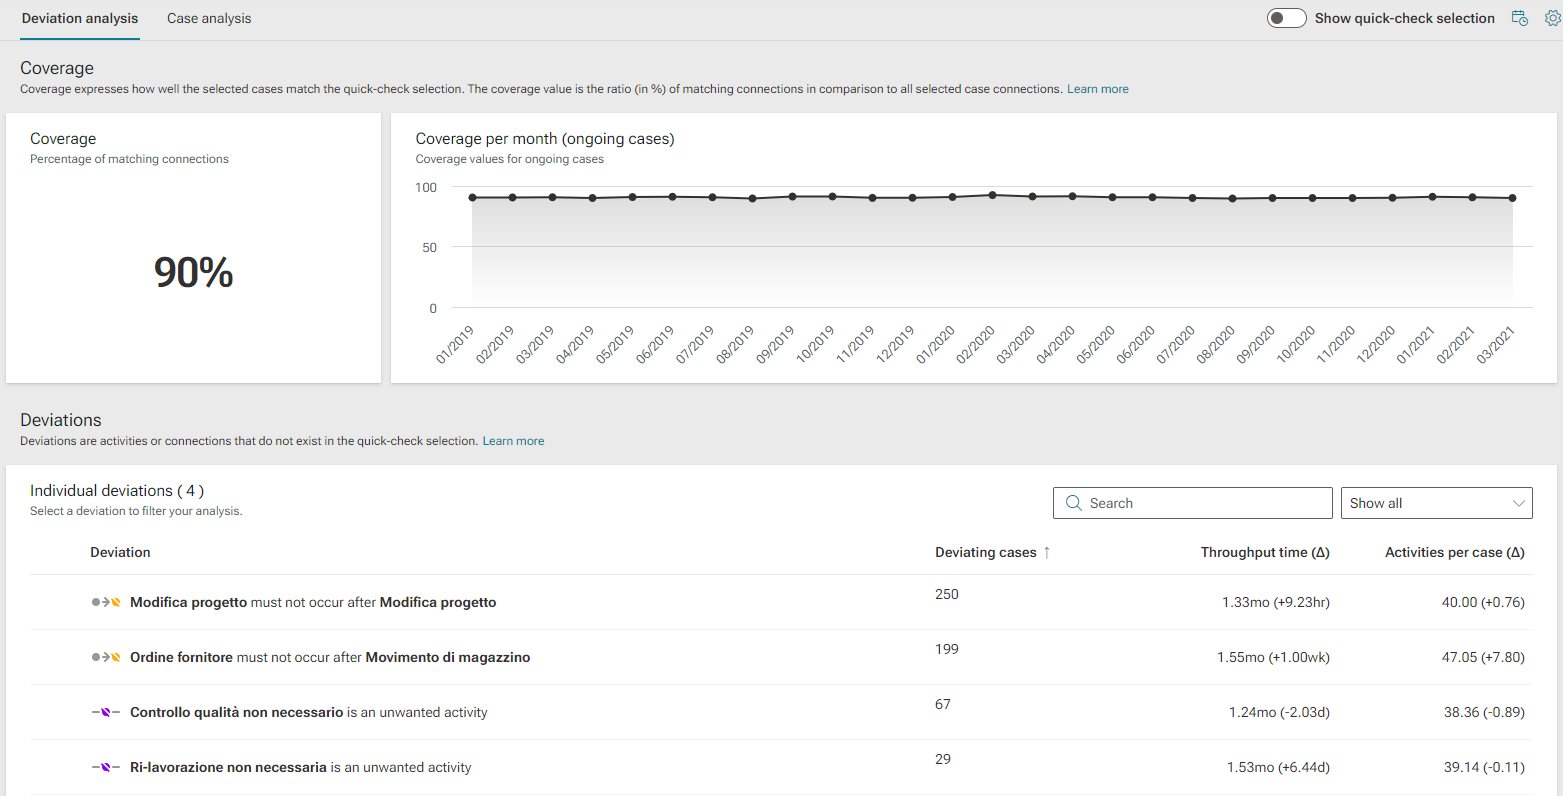
\includegraphics[width=\textwidth]{imgARIS/Simulazione/QuickCheck1Simulazione.png}
    \caption{Panoramica delle deviazioni nel processo}
    \label{fig:quick-check-1}
\end{figure}
La sezione dedicata alla Deviation Analysis mette in evidenza la copertura del processo, cioè la percentuale di connessioni che corrispondono a quelle previste nel "quick-check". In questo caso, vediamo un valore del 90\%, che indica una buona aderenza al flusso previsto, ma segnala comunque la presenza di alcune deviazioni. Questo dato viene accompagnato da un grafico che traccia la copertura mensile dei casi, fornendo una visione temporale dell'aderenza al processo, utile per individuare eventuali cambiamenti o miglioramenti nel tempo.\\
L'elemento chiave della schermata è però la parte relativa alle deviazioni, che elenca le attività o connessioni che non corrispondono alla configurazione di controllo. In questo esempio, si vedono quattro deviazioni, ognuna delle quali mostra il numero di casi coinvolti, il tempo di attraversamento e il numero di attività per caso. La funzionalità di Quick Check permette quindi di filtrare e analizzare ogni singola deviazione, evidenziando quanto queste influiscano sull'efficienza complessiva del processo, come nel caso di una "Modifica progetto" che non dovrebbe avvenire consecutivamente. Attraverso questi dati, si può subito capire l'impatto di ogni deviazione in termini di tempo extra e complessità aggiuntiva.\\

\begin{figure}[H]
    \centering
    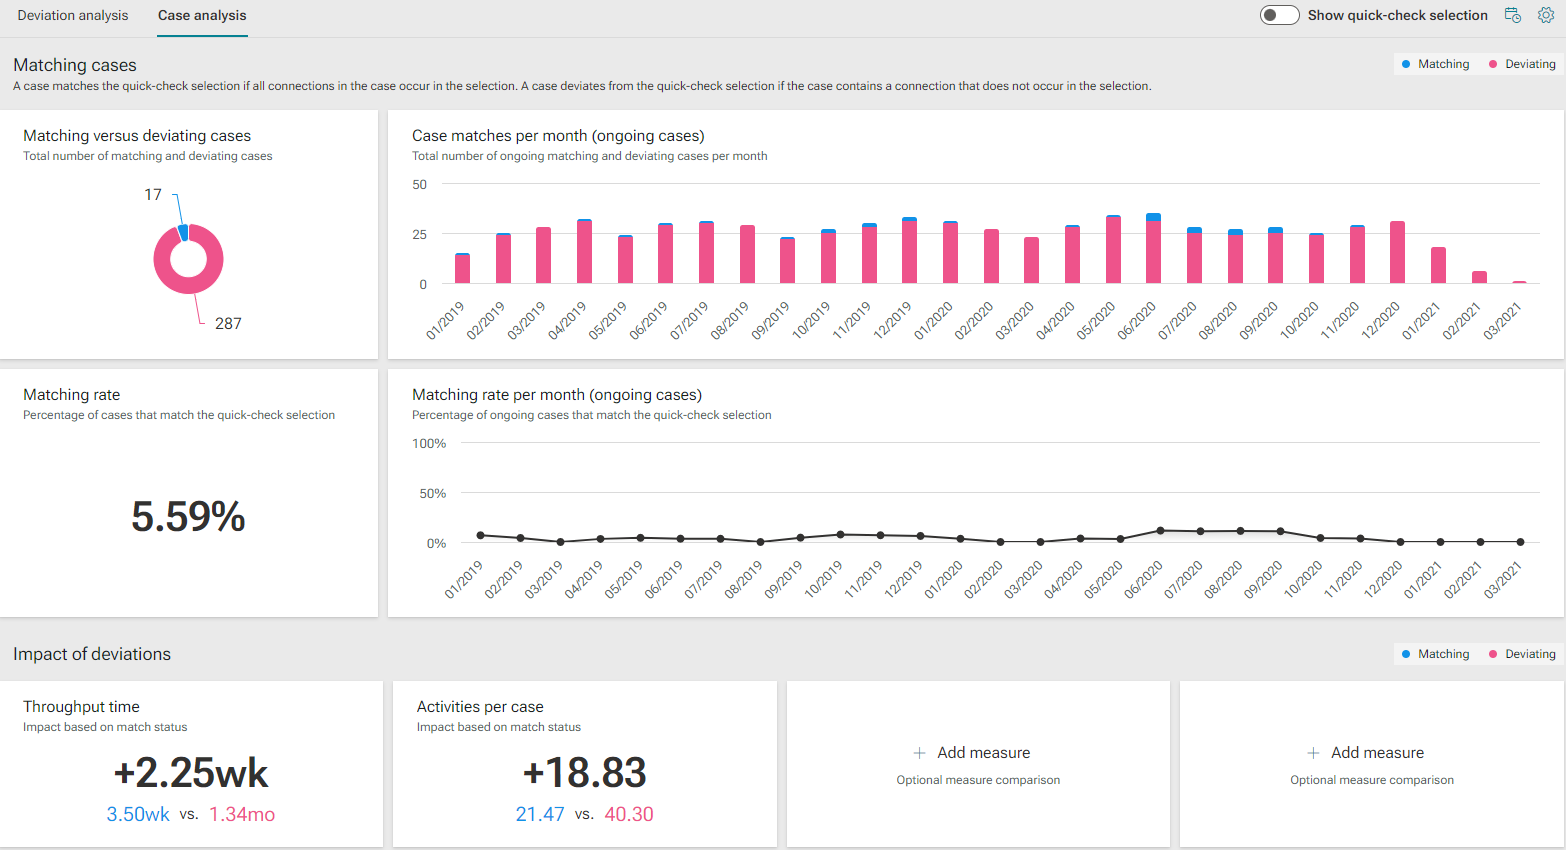
\includegraphics[width=\textwidth]{imgARIS/Simulazione/QuickCheck2Simulazione.png}
    \caption{Analisi dei casi conformi e devianti}
    \label{fig:quick-check-2}
\end{figure}
Nell'analisi dei casi l’attenzione si sposta sul confronto tra i casi che rispettano le aspettative del quick-check e quelli che invece si discostano. L'infografica a torta nella parte superiore indica immediatamente la distribuzione tra i casi conformi e quelli che deviano, con una maggioranza evidente di casi devianti. Il Matching rate, che è al 5,59\%, evidenzia che solo una piccola percentuale dei casi segue effettivamente il percorso previsto. Questo è uno degli elementi centrali della funzionalità: permettere di misurare in modo chiaro la conformità del processo e capire quanto spesso le eccezioni o le deviazioni avvengano.\\
Un aspetto interessante è anche la visualizzazione dell'impatto delle deviazioni. In basso, si può osservare come le deviazioni incidano sui tempi di attraversamento e sul numero di attività per caso. Ad esempio, vediamo che le deviazioni aggiungono in media 2,25 settimane al throughput time, e aumentano il numero di attività per caso di quasi 19 attività. Questo permette di quantificare l'effetto delle anomalie, trasformando l'analisi delle deviazioni in uno strumento concreto per valutare i costi operativi associati ai percorsi non conformi.

\section{Implementazioni pratiche: dati reali}
\subsection{Struttura dei dati}
Per testare le funzionalità dello strumento di process mining di Microsoft, è stata scelta una tabella del database ERP di un'azienda produttrice di porte. Nello specifico, si è deciso di utilizzare la tabella che registra i movimenti di magazzino, poiché ogni movimento rappresenta un'attività nel processo di produzione. Inoltre, questa tabella è ricca di dati, offrendo così un'ampia base di informazioni per l'analisi.\\
Le colonne della tabella sono le seguenti:
\begin{itemize}
    \item \custombold{NRO\_REGISTRAZIONE}: numero di registrazione del movimento di magazzino;
    \item \custombold{DATA\_MOVIMENTO}: data di creazione del movimento di magazzino;
    \item \custombold{COD\_CAUSALE}: codice di riferimento della causale del movimento di magazzino;
    \item \custombold{MASTRO}: codice mastro del cliente o del fornitore del movimento;
    \item \custombold{PARTITARIO}: codice partitario del cliente o del fornitore del movimento;
    \item \custombold{NRO\_DOCUMENTO}: indica il numero del documento che ha originato il movimento;
    \item \custombold{DATA\_DOCUMENTO}: indica la data del documento che ha orignato il movimento;
    \item \custombold{NRO\_REGIST\_MOV\_ABB}: numero registrazione del movimento abbinato;
    \item \custombold{COD\_MAGAZZINO}: codice del magazzino da proporre a livello di riga;
    \item \custombold{COD\_VALUTA}: valuta alla quale è stato eventualmente valorizzato il movimento;
    \item \custombold{CAMBIO}: valore del cambio del movimento;
    \item \custombold{MASTRO\_AGENTE}: mastro agente collegato al movimento;
    \item \custombold{NRO\_ORDINE}: riferimento all`ordine nel movimento;
    \item \custombold{NRO\_RIF\_CONTAB\_FATTURA}: numero di riga della registrazione del movimento contabile della fattura legato al documento che ha generato il movimento di magazzino;
    \item \custombold{RIGA\_RIF\_CONTAB\_FATTURA}: riga della registrazione contabile della fattura a cui il movimento di magazzino si riferisce;
    \item \custombold{RIF\_LOTTO}: non utilizzato;
    \item \custombold{NRO\_FT}: acquisti: numero della fattura attribuito dal fornitore; vendite: Sez/Nro fattura;
    \item \custombold{DATA\_FT}: acquisti: data della fattura attribuita dal fornitore; vendite: data fattura;
    \item \custombold{RIF\_ANNO\_DOC}: questo attributo e i seguenti contengono gli estremi del documento che ha generato il documento di magazzino;
    \item \custombold{RIF\_TIPO\_DOC}
    \item \custombold{RIF\_NRO\_DOC}
    \item \custombold{AMBITO\_RIF\_DOC}: questo attributo definisce se il movimento di magazzino e stato inserito manualmente oppure se e stato generato da un documento di vendita o di acquisto;
    \item \custombold{DATA\_COMP}: data di competenza della registrazione.
    \item \custombold{RIF\_MOV\_MAG\_SCAR\_COMP}: riferimento all'eventuale movimento di scarico componenti;
    \item \custombold{ALTRI\_RIF\_TEST}: campo descrittivo a disposizione dell'utente;
    \item \custombold{TXT\_A\_DISP\_1}: testo a disposizione 1;
    \item \custombold{TXT\_A\_DISP\_2}: testo a disposizione 2;
    \item \custombold{TXT\_A\_DISP\_3}: testo a disposizione 3;
    \item \custombold{DATA\_A\_DISP\_1}: data  a disposizione 1;
    \item \custombold{DATA\_A\_DISP\_2}: data  a disposizione 2;
\end{itemize}
Inoltre, è stata associata a questa tabella un'altra tabella contenente le informazioni sulle causali di magazzino, necessarie per etichettare i dati della prima tabella rendendoli più facilmente leggibili. La struttura della tabella delle causali di magazzino è la seguente:
\begin{itemize}
    \item \custombold{COD\_CAUSALE}: codice causale;
    \item \custombold{DESCRIZIONE}: descrizione;
    \item \custombold{MAGAZZ\_DEFAULT}: indica il magazzino da proporre come default per i movimenti di magazzino che appartengono alla causale;
    \item \custombold{MAGAZZ\_COLL\_DEFAULT}: indica il magazzino collegato da proporre come default per i movimenti di magazzino che appartengono alla causale;
    \item \custombold{SE\_REG\_FISCALE}: indica se il movimento deve essere stampato nel registro fiscale o meno;
    \item \custombold{SE\_QUANTITA}: indica se la valorizzazione della quantita e obbligatoria con il programma di gestione movimenti di magazzino (Y/N);
    \item \custombold{SE\_PREZZO}: indica se la valorizzazione di prezzo e valore e obbligatoria con il programma di gestione movimenti di magazzino (Y/N);
    \item \custombold{SE\_SCONTO}: indica se la valorizzazione dello sconto e obbligatoria con il programma di gestione movimenti di magazzino (Y/N);
    \item \custombold{COD\_CAUSALE\_ULT\_PREZZO}: indica il tipo di prezzo di movimento proposto come default dal programma di gestione movimenti (prezzo medio, ultimo prezzo di carico, ...);
    \item \custombold{COD\_CAUSALE\_DB}: collegamento tra magazzino e produzione;
    \item \custombold{INPUT\_CLI\_FORN\_TUTTI}: indica per quali conti è valida la causale se per clienti, fornitori o tutti;
    \item \custombold{COD\_TIPO\_RIEPILOGO}: questo attributo indica se il movimento è di Esistenza iniziale, di Carico o di Scarico;
    \item \custombold{EVEN\_COD\_CAUSALE\_ABB}: nel caso sia presente la causale abbinata significa che la causale di movimentazione prevede un movimento abbinato;
    \item \custombold{ART\_DIV\_SU\_CAUS\_ABB}: indica che l`articolo movimentato dalla causale abbinata e diverso dall`articolo movimentato dalla causale corrente;
    \item \custombold{SE\_VALIDO\_PER\_PREZ\_MED}: includere o meno il movimento nel calcolo del prezzo medio dell`articolo;
    \item \custombold{AGG\_DATI\_FORNITORE}: Non gestito;
    \item \custombold{SE\_DA\_FATT}: indica se il documento di vendita corrispondente al movimento e da fatturare o meno;
    \item \custombold{INTRA\_COD\_TRANSAZIONE}: codice transazione (per intrastat);
    \item \custombold{SE\_GEST\_LOTTI}: indica se è prevista la gestione a lotti;
    \item \custombold{SE\_NON\_MOV\_MAG}: indica se il magazzino deve essere o meno movimentato;
    \item \custombold{TIPO\_ART\_ABIT}: tipo articolo abituale per movimenti manuali;
    \item \custombold{PROP\_ULT\_PZZO}: tipo proposta;
    \item \custombold{SE\_ANALITICA}: indica se la valorizzazione dei riferimenti contabilita analitica (voce di spesa, centro di costo e commessa) è obbligatoria con il programma di gestione movimenti di magazzino (Y/N);
    \item \custombold{TIPO\_COSTO\_ULT\_PREZZO}: tipo costo per prezzo di default;
    \item \custombold{SE\_VALIDO\_PER\_PREZ\_PRJ}: includere o meno il movimento nel calcolo del prezzo medio di progetto;
    \item \custombold{COD\_CAUS\_MOV\_PRJ}: causale di movimentazione della contabilita di progetto;
    \item \custombold{SE\_VAL\_MOV\_DOCUMENTO}: indica se il movimento di magazzino generato da documento deve essere valorizzato (Y/N);
    \item \custombold{SE\_PRZ\_MEDIO\_NO\_VAL}: indica se il movimento di magazzino viene considerato per il calcolo del prezzo medio anche se privo di valore (Y/N).
\end{itemize}
A causa della limitazione della licenza dello strumento di process mining, l'analisi è stata eseguita su un subset della tabella, limitato a un massimo di 100 MB di dati. Questo implica che non tutti i dati disponibili nel database sono stati utilizzati, ma solo quelli necessari e sufficienti per condurre l'analisi.
\end{document}
